\subsection{Development}
\begin{figure}
    \centering
    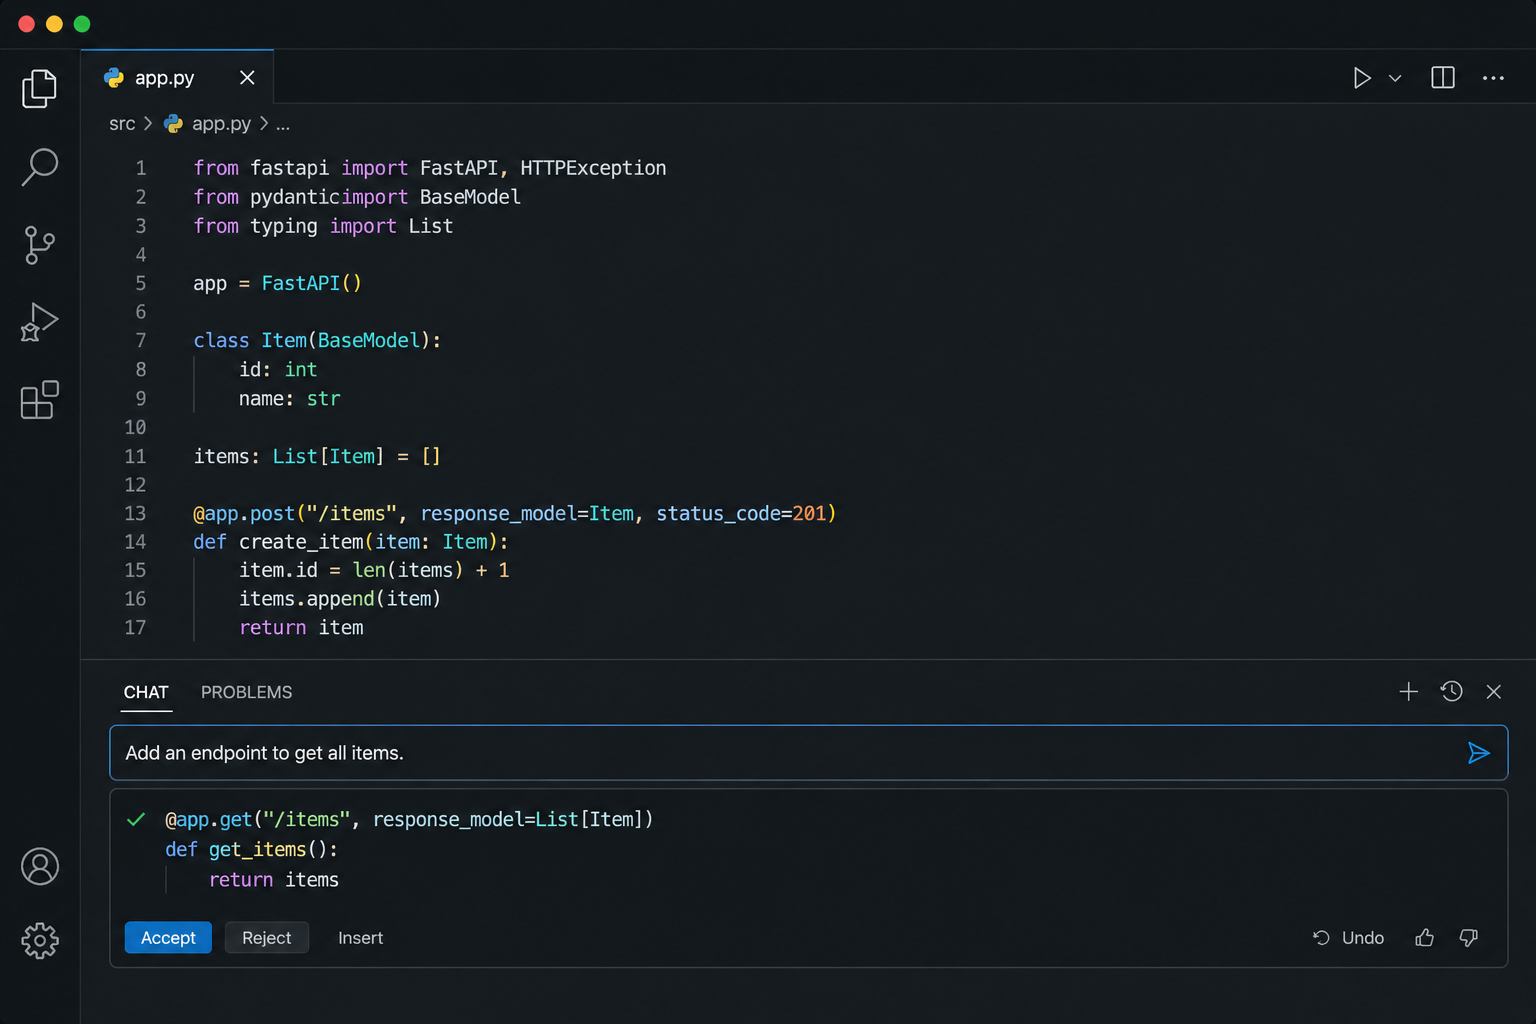
\includegraphics[width=\columnwidth]{content/figures/dev-inline-chat.png}
    \caption{An example of an inline chat interface integrated into a code editor, allowing developers to interact with an LLM for real-time code suggestions and debugging assistance.}
    \label{fig:dev:dev-inline-chat}
\end{figure}
The development phase of the Software Development Life Cycle (SDLC) focuses on translating requirements into working code through design, implementation, and integration. Traditionally, this stage relies heavily on developer expertise, iterative problem-solving, and debugging practices. The continuous evolution of software development practices has led to a growing interest in the integration of cutting edge technology to enhance developer productivity \cite{chen2021evaluatingllm}. One such technology that has garnered considerable attention is the utilization of Large Language Models (LLMs) within Integrated Development Environments (IDEs) \cite{chen2023vscuda,daye2023inide}. These models can accelerate implementation (Figure \ref{fig:dev:dev-inline-chat}) and reduce cognitive load by providing instant suggestions and alternatives, but they also influence how developers approach problem-solving, often shifting effort from writing code to validating and refining AI-generated outputs.

\subsubsection{Code Generation From Natural Language}
\citet{stages_dev_agarwal2024copilot} evaluated how LLMs translate natural language intent into executable code within an IDE-centric workflow. Their methodology involved selecting real-world methods from GitHub repositories, providing the model with the function signature, docstring, and surrounding file context, and prompting it to generate the method body. The generated code is then reintegrated into the original project and evaluated using syntax correctness and test pass rate, where the entire test suite is executed to verify functional behavior. This ensures that evaluation reflects realistic development conditions, where generated code must interact correctly with existing components rather than operate in isolation.
\begin{table}[h]
    \centering
    \begin{tabular}{@{}llcc@{}}
        \\
        \toprule
        \textbf{Language}           & \textbf{Model} & \textbf{Syntax }     & \textbf{Bugs}  \\
                                    &                & \textbf{Correctness} & \textbf{Fixed} \\
        \toprule
        \multirow{3}{*}{Python}     & GPT-4          & 96\%                 & 74\%           \\&  GPT-3.5& 93\% & 68\%\\&CodeLlama & 88\% & 39\%\\
        \toprule
        \multirow{3}{*}{Javascript} & GPT-4          & 92\%                 & 81\%           \\&  GPT-3.5 & 85\% & 74\%\\&CodeLlama & 39\% & 26\%\\
        \toprule
        \multirow{3}{*}{Typescript} & GPT-4          & 83\%                 & 75\%           \\&  GPT-3.5 & 74\% & 75\%\\&CodeLlama & 70\% & 30\%\\
        \toprule
        \multirow{3}{*}{C\#}        & GPT-4          & 98\%                 & 58\%           \\&  GPT-3.5  & 96\% & 65\%\\&CodeLlama  & 84\% & 50\%\\
        \bottomrule
    \end{tabular}
    \caption{\citet{stages_dev_agarwal2024copilot} evaluated the effectiveness of LLMs in generating syntactically correct code and fixing bugs across multiple programming languages. The results show that while LLMs can produce high rates of syntactically correct code, their ability to fix bugs varies significantly}
    \label{tab:fix_results}
\end{table}
The findings show that LLMs are generally effective at producing syntactically valid code and can often satisfy functional requirements when sufficient context and test coverage are provided. However, several limitations emerge: generated code may fail hidden edge cases not covered by tests, may rely heavily on prompt quality and context completeness, and can struggle with complex dependencies across files. Additionally, correctness is not guaranteed even when code appears plausible, emphasizing the gap between surface-level generation and true semantic understanding. These results highlight that while LLMs significantly accelerate initial implementation, their outputs require systematic validation and integration checks to ensure reliability in real-world development scenarios.

